%% Casos de uso %%

\documentclass[11pt, a4paper, twoside, titlepage]{article}
\usepackage[utf8x]{inputenc}
\usepackage[T1]{fontenc}
\usepackage{lmodern}
\usepackage[spanish]{babel}
\usepackage[none]{hyphenat}
\usepackage{fancyhdr}
\usepackage{isdiedral}
\usepackage{anysize}
\usepackage{graphicx}
\usepackage{float}
\usepackage{rotating}
\usepackage[colorlinks, linkcolor=black]{hyperref}

% Nombre del documento (para futuras referencias)
\newcommand*{\doctitle}{Casos de uso}

%%% Configuraciones %%%
\marginsize{2cm}{2cm}{2cm}{2cm}

% Usa como familia tipográfica por defecto "Sans"
\renewcommand{\familydefault}{\sfdefault}

% Establece la profundidad de niveles de sección que aparece en el TOC
\setcounter{tocdepth}{3}

% Configura los encabezados y pies de paǵina
\encabezadodiedral{\doctitle}
\pagestyle{fancy}
\renewcommand*{\thepage}{\sffamily \roman{page}}

\title{\doctitle\\\textsl{Airline Common Environment}}
\author{Grupo Diedral}

% Metadatos del pdf
\hypersetup{
pdfinfo={
	Author={Grupo Diedral},
	Title={\doctitle},
	Subject={Airline Common Environment},
	Keywords={Casos de uso;Airline Common Environment;Ingeniería del Software}
}
}

\begin{document}
	% Historial de cambios
	\begin{tablacambios}
		1 & 13 de diciembre de 2013 & CAF, NAH, SBC, JCP, RRC & Continuación
	\end{tablacambios}
	\newpage

	% Página de título
	\portadaace{\doctitle}

	% Índice
	\tableofcontents
	\listoffigures
	
	% Prólogo
	\begin{prologo}
		Este documento, bla, bla, bla\ldots
	\end{prologo}

	% Cada caso de uso se puede escribir en un archivo aparte e importar
	% usando  "include"  que  utiliza  necesariamente  una  página (para
	% evitarlo se puede usar "input" en su lugar).
	\section{Casos de uso}
	
	% Gestión interna
	\subsection{Gestión interna} \vspace{.5cm}
	\iniciarnumeraciondiedral

	\begin{sidewaysfigure}	% LaTex lo coloca donde le parece (como debe hacer)
		\hspace*{-2cm}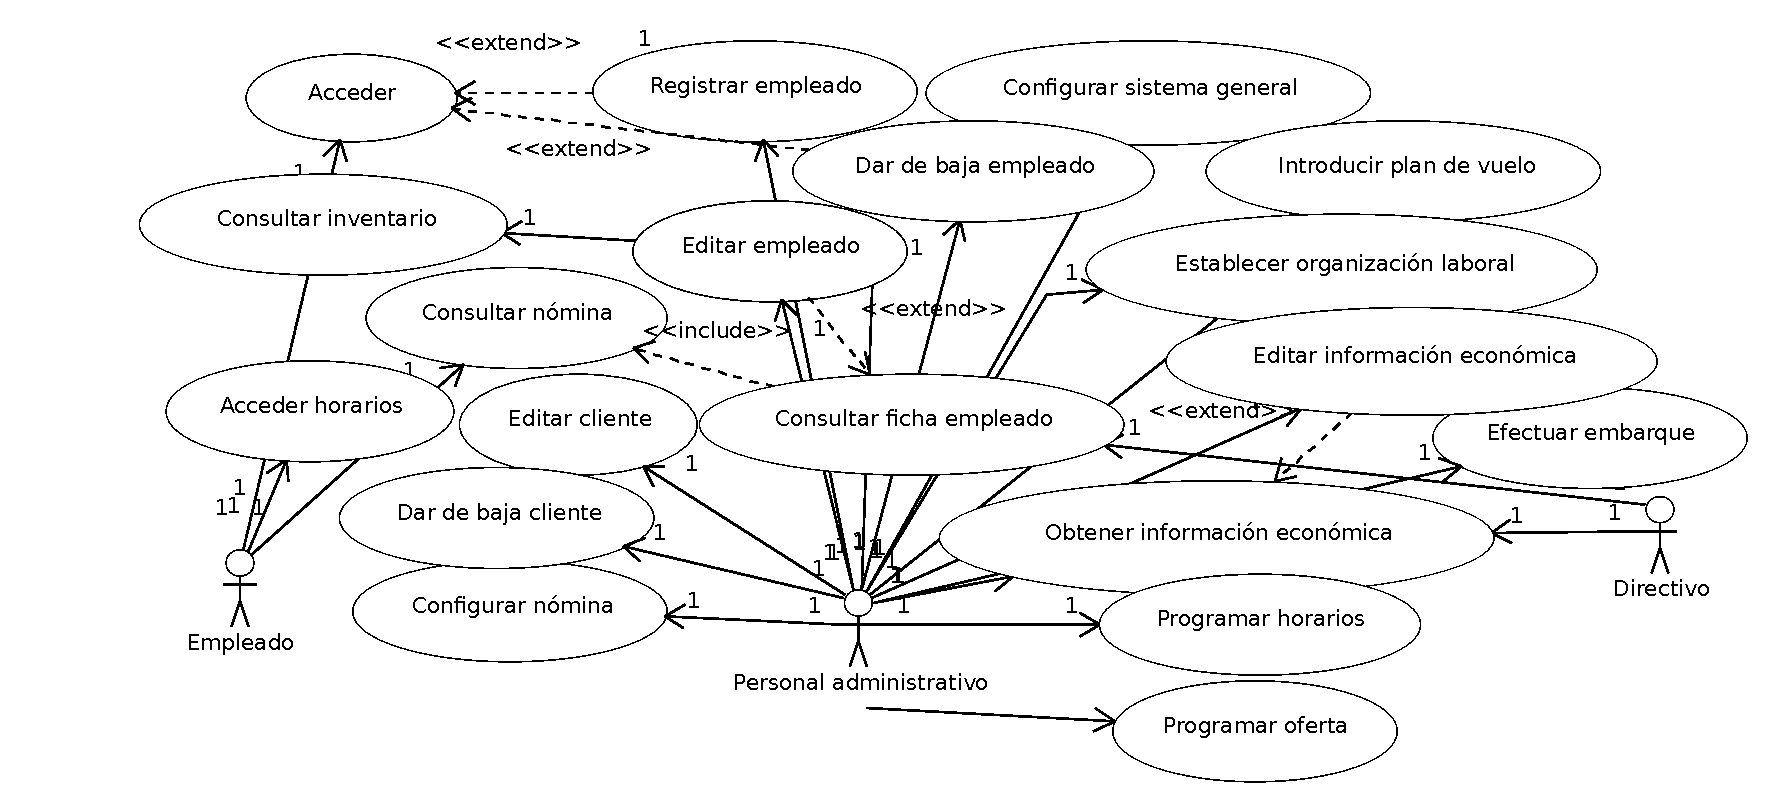
\includegraphics[scale=.9]{diagramas/gestioninterna1.pdf}
		\caption{Diagrama de gestión interna (administrativo)}
	\end{sidewaysfigure}

	\begin{sidewaysfigure}
		\hspace*{0cm}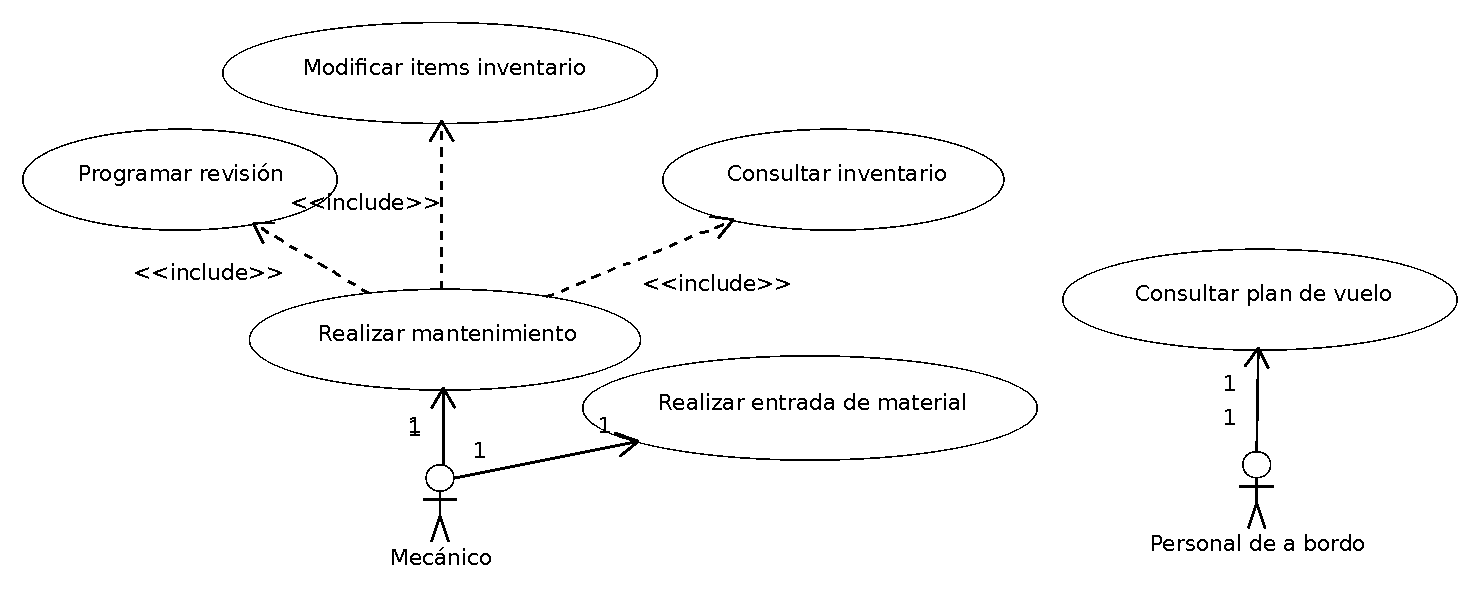
\includegraphics[scale=.9]{diagramas/gestioninterna2.pdf}
		\caption{Diagrama de gestión interna (mecánico y personal de a bordo)}
	\end{sidewaysfigure}

	% Revisado por Juanan el día 12/03/2013

\srsfuncion{Acceder}
	Función que permite al empleado de la compañía aérea identificarse en el sistema para así poder hacer uso de las funciones que ofrece de acuerdo a las limitaciones establecidas para su puesto de trabajo (\gls{Login}).
		
	\begin{enumerate}
		\item \textit{Prioridad}: alta.
		\item \textit{Entradas}
		\begin{enumerate}
			\item El identificador de usuario deberá introducirse para poder acceder, además de la contraseña personal de cada usuario.
			\item En el campo contraseña serán válidos los caracteres ASCII imprimibles.
		\end{enumerate}
		\item \textit{Flujo de operaciones}
		\begin{enumerate}
			\item Se muestran por pantalla dos campos a rellenar: uno para introducir el id del usuario y otro para escribir la contraseña.
			\item El usuario para identificarse y acceder al sistema despues de haber introducido los datos requeridos selecciona la opción acceder.
		\end{enumerate}
		\item \textit{Respuesta a situaciones no previstas}
		\begin{enumerate}
			\item Si algún campo introducido no es válido, se indica y se da la opción de introducirlo de nuevo. Existe un límite de 5 intentos de acceso fallido en un periodo de tiempo corto (15 minutos).
		\end{enumerate}
	
\end{enumerate}

	\srsfuncion{Registrar empleado} \label{fun:registrarempleado}
	Esta función debe permitir añadir un nuevo empleado a la base de datos del sistema de la compañía aérea.

\begin{enumerate}
	\item \textit{Prioridad}: alta.
	\item \textit{Entradas}
	\begin{enumerate}
		\item El nombre y apellidos del empleado deberán contener únicamente carácteres alfabéticos latinos, acentuados o no, y espacios.
		\item El código de identificación personal debererá cumplir los requisitos que se establecen en \nameref{srs:idpersonal}.
		\item La dirección se compondrá de un tipo de vía (calle, avenida, paseo), un nombre válido, un número de portal (entero mayor estricto que 0), escalera (izquierda, derecha, centro o nada), piso (entero mayor estricto que 0 o letra B) y puerta (letra o entero mayor estricto 0).
		\item El número de teléfono deberá ser una secuencia de 9 dígitos.
		\item El puesto de trabajo deberá seleccionarse de una lista finita fijada con anterioridad.
	\end{enumerate}
	\item \textit{Flujo de operaciones}
	\begin{enumerate}
		\item Se muestra por pantalla una tabla con los datos personales del empleado que deben ser completados (nombre, apellidos, código de identificación peronal, dirección, teléfono, puesto de trabajo que ocupará dentro de la empresa y otros datos personales opcionales para completar el registro).
		\item El encargado del registro deberá confirmar el alta pulsando en el botón \verb|Guardar|.
		\item Se generá un nuevo nombre de usuario y una contraseña, que se asignarán a la cuenta de correo interna del usuario.
		\item Se imprime entonces una ficha con los datos de la cuenta para el empleado.
	\end{enumerate}
	\item \textit{Respuesta a situaciones no previstas}
	\begin{enumerate}
		\item Si no se puede acceder a la base de datos para almacenar la información: se muestra un mensaje de error por pantalla informando de que el registro no ha podido completarse y el usario no ha sido añadido a la base de datos. Se vuelve a la página principal del sistema.
		\item Si algún campo introducido no es válido: se señalan los campos erróneos y se da la opción de volver a introducir los datos.
	\end{enumerate}

\end{enumerate}

	% Caso de uso: verificar registro empleado.
% Obs: para escribir comas en el texto del primer parámetro se han de encerrar entre {}.

\casodeuso{
	% Nombre del caso de uso
	nombre=Verificar el registro de un empleado.,
	% Objetivo
	objetivo=Establece una nueva cuenta de usuario como válida y totalmente operativa.,
	% Entradas
	entradas={Los datos del usuario previamente registrado, incluyendo su futuro puesto de trabajo en la compañía.},
	% Precondiciones
	precondiciones={El nuevo usuario ha sido registrado correctamente en el sistema, el empleado de Recursos Humanos tiene los permisos necesarios para realizar la operación y ha accedido a la opción \textit{Verificar registro empleado}.},
	% Salidas
	salidas={Confirmación de la operación, si procede.},
	% Postcondiciones en caso de éxito
	postexito={La cuenta del usuario queda verificada y, por tanto, pasa a estar activa y totalmente operativa.},
	% Postcondiciones en caso de error
	posterror=La cuenta del usuario permanece inactiva.,
	% Actores
	actores=El personal del departamento de intervención y la base de datos.,
}{
	% Tabla de secuencia normal del caso de uso
	\begin{tablasecuencias}
		1 & Se extrae de la base de datos del sistema la información de la cuenta del usuario. Si error S-1. \\
		2 & Se muestran los datos por pantalla y se comprueba que sean correctos. Si error S-2.\\
		3 & Se verifica la cuenta del usuario y se modifica en la base de datos. Si error S-3.\\
		4 & Se muestra por pantalla un mensaje de confirmación de la operación.
	\end{tablasecuencias}
}{
	% Tabla de secuencia con errores del caso de uso
	\begin{tablasecuencias}
		S-1 & No se ha podido conectar con la base de datos. Mostrar un mensaje de error por pantalla y volver a la página principal de la aplicación.\\
		S-2 & Alguno de los datos de la cuenta es erróneo, o se han concedido al usuario permisos que no se corresponden a su función en la compañía. El empleado del departamento de intervención cancela la operación e informa al personal administrativo para que contacten con el futuro empleado y se proceda de nuevo a su registro.\\
		S-3 & No se ha podido acceder a la base de datos. Se cancela la operación, se muestra un mensaje de error por pantalla y vuelve a la página principal de la aplicación.\\
	\end{tablasecuencias}
}



	% Caso de uso: consultar ficha empleado.
% Obs: para escribir comas en el texto del primer parámetro se han de encerrar entre {}.

% Revisado por Cristina y Juanan el día 11/03/2013

\casodeuso{
	% Nombre del caso de uso
	nombre=Consultar ficha empleado,
	% Objetivo
	objetivo={Mostrar la lista de empleados de la compañía, permitiendo buscar y filtrar resultados, así como información detallada de cada empleado en particular.},
	% Entradas
	entradas={Opcionalmente, campos de búsqueda.},
	% Precondiciones
	precondiciones=El operador de la aplicación tiene credenciales que le habilitan para realizar dicha operación.,
	% Salidas
	salidas=Lista de empleados e información detallada sobre el seleccionado.,
	% Postcondiciones en caso de éxito
	postexito=No se realiza ningún cambio en el sistema.,
	% Postcondiciones en caso de error
	posterror=No se realiza ningún cambio en el sistema.,
	% Actores
	actores={Los directivos, empleados de recursos humanos y la base de datos.}.
}{
	% Tabla de secuencia normal del caso de uso
	\begin{tablasecuencias}
		1 & Se extrae de la base de datos del sistema el listado de empleados. Si error S-1.\\
		2 & Se muestra por pantalla la lista de empleados.\\
		3 & El usuario puede filtrar los resultados y buscar empleados según diferentes criterios, como tipo de empleado, duración en la empresa, departamentos, etc.\\
		4 & Se selecciona un empleado.\\
		5 & Se muestra la información detallada del empleado. Si error S-1.
	\end{tablasecuencias}
}{
	% Tabla de secuencia con errores del caso de uso
	\begin{tablasecuencias}
		S-1 & No se puede conectar con la base de datos, se muestra un mensaje de error por pantalla dando la opción de reintentar o volver al menú principal de la aplicación.
	\end{tablasecuencias}
}

	
% Revisado por Cristina el día 12/03/2013

\srsfuncion{Editar empleado}
	Esta función permite modificar la información de la ficha de un empleado.

	\begin{enumerate}
		\item \textit{Prioridad}: media.
		\item \textit{Entradas}
		\begin{enumerate}
			\item Las opciones que admiten modificación son: nombre, apellidos, foto, número de teléfono, NIF, número de seguridad social, contraseña de acceso, domicilio, dirección de correo electrónico y número de cuenta bancaria.
			\item La contraseña está formada por entre 8 y 16 caracteres alfanuméricos.
			\item El \gls{NIF} debe ser verificado algorítmicamente.
			\item El código postal del domicilio está compuesto por 5 cifras.
			\item Se verifica mediante el dígito de control la validez del número de cuenta.
		\end{enumerate}
		\item \textit{Flujo de operaciones}
		\begin{enumerate}
			\item El administrativo modifica al menos uno de los diferentes campos.
			\item El empleado confirma los cambios.
			\item Si se verifican los datos modificados se confirma la operación, actualizando la \gls{base_de_datos}.
			\item Se muestra la ficha de empleado actualizada.
		\end{enumerate}
		\item \textit{Respuesta a situaciones no previstas}
		\begin{enumerate}
			\item Si algún campo introducido no es válido, se indica y se da la opción de introducirlo de nuevo.
			\item Si no se puede acceder o modificar a la base de datos, se muestra un mensaje de error y se da la opción de reintentar o abortar el proceso.
		\end{enumerate}
	\end{enumerate}

	
% Revisado por Cristina el día 12/03/2013

\srsfuncion{Dar de baja empleado}
	Esta función permite dar de baja a un empleado, eliminando su información personal de acuerdo a la legislación vigente y derogando las autorizaciones de acceso al sistema y las instalaciones.
	
	\begin{enumerate}
		\item \textit{Prioridad}: alta.
		\item \textit{Entradas}
		\begin{enumerate}
			\item No hay entradas.
		\end{enumerate}
		\item \textit{Flujo de operaciones}
		\begin{enumerate}
			\item El administrativo confirma que quiere realizar la operación dar de baja con el cliente\break	 seleccionado.
			\item El empleado dado de baja pierde inmediatamente todo acceso al sistema y su información personal se elimina de la base de datos de acuerdo a la legislación vigente.
			\item Se muestra un mensaje confirmando la operación.
		\end{enumerate}
		\item \textit{Respuesta a situaciones no previstas}
		\begin{enumerate}
			\item Si no se puede establecer conexión con la base de datos, se muestra un mensaje de error y se da la opción de reintentar o abortar el proceso.
		\end{enumerate}
	\end{enumerate}

	\srsfuncion{Configurar el sistema}  \label{fun:configSystem}
	Esta función permite modificar ciertos parámetros de la configuración general del sistema.

	\begin{enumerate}
		\item \textit{Prioridad}: media
		\item \textit{Usuarios}: personal administrativo o de los servicios informáticos debidamente autorizado.

		\item \textit{Entradas} \\

			Los parámetros configurables se restringirán a los indicados a continuación. Téngase en cuenta que algunos conllevan una considerables cambios difícilmente aplicables, son de uso totalmente infrecuente y requieren la supervisión activa del usuario.
			\begin{enumerate}
				\item Fecha y hora del servidor central. Su aplicación no será inmediata ya que requerirá procesos de sincronía con los equipos conectados y probablemente el reinicio de ciertos componentes del sistema.
				\item Nombre de la compañía. El nombre que aparece en los informes generados por la aplicación, así como en las ventanas de su interfaz.
				\item Moneda. Tipo monetario en el que se expresan los importes comerciales y la información económica de la empresa. Su implantación no es inmediata pues puede requerir conversión de los datos en uso o históricos. La guía del usuario será necesaria para la aplicación de este cambio.
				\item Criterio de ordenación por defecto para cada caso de uso que presente información ordenada\footnote{\textit{Consultar ficha empleado}, \textit{Consultar ficha cliente}, \textit{Establecer organización laboral}\ldots}. Permitirá seleccionar entre los criterios de ordenación disponibles para cada caso de uso aquél que se tomará por omisión. De aplicación inmediata.
			\end{enumerate}

			Las entradas deberán atenerse a lo siguiente:
			\begin{enumerate}
				\item No se podrán establecer configuraciones inválidas o que vayan a causar error en otras funciones.
				\item La configuración del sistema no puede quedar dañada por la modificación del empleado.
			\end{enumerate}

		\item \textit{Flujo de operaciones}
		\begin{enumerate}
			\item Mostrar los valores previos de los parámetros configurables.
			\item Se modifican los campos que se quieren reconfigurar en el sistema.
			\item El usuario, una vez satisfecho con los cambios realizados, confirma su modificación. Se comprueba la coherencia de los datos antes del envío. 
			\item Una vez que la configuración ha sido establecida con éxito, se mostrará un mensaje por pantalla indicando que se ha modificado la configuración del sistema general.
			\item Los cambios que así lo requieran presentarán al usuario pantallas para afinar el proceso de consolidación de los ajustes. Además si la implantación requiriese un determinado tiempo para llevarse a cabo se monitorizará el proceso. Algunos cambios pueden requerir el reinicio del sistema o alguno de sus componentes para llegar a efecto.
		\end{enumerate}
		\item \textit{Respuesta a situaciones no previstas}
		\begin{enumerate}
		  \item Si no se ha podido acceder a la base de datos del sistema para poder modificar así la configuración, se mostrará un mensaje por pantalla indicando que en estos momentos no se puede realizar una configuración del sistema. Se le mandará al menú principal.
			\item Si los datos introducidos en los campos son incorrectos, se marcarán dichos incorrectos y se mostrará un mensaje de error indicando un breve resumen de los detalles por los que esos campos son incorrectos.
		\end{enumerate}

	\end{enumerate}

	% Caso de uso: establecer organización laboral.
% Obs: para escribir comas en el texto del primer parámetro se han de encerrar entre {}.

\casodeuso{
	% Nombre del caso de uso
	nombre=Establecer organización laboral,
	% Objetivo
	objetivo={Establece las configuraciones generales sobre la organización laboral de la compañía, como secciones y puestos de trabajo, detallando la información relacionada (salario base\dots) y fijando los privilegios de acceso dentro de la aplicación.},
	% Entradas
	entradas={Las valores correspondientes a esas configuraciones, como por ejemplo: nombre, descripción, salario base, privilegios\dots},
	% Precondiciones
	precondiciones={El operador de la aplicación está debidamente registrado y posee credenciales que le habilitan para realizar esta operación.},
	% Salidas
	salidas={Valor final de los parámetros configurados.},
	% Postcondiciones en caso de éxito
	postexito=Todas las utilidades de la aplicación que requieran de estas configuraciones podrán disfrutar de ellas.,
	% Postcondiciones en caso de error
	posterror={El sistema central no habrá sufrido cambios.},
	% Actores
	actores={Personal de administración, \textit{Recursos Humanos} y \textit{Servicios Informáticos}.},
}{
	% Tabla de secuencia normal del caso de uso
	\begin{tablasecuencias}
		1 & Se muestran sendas listas de categorías obtenidas del servidor central, permitiendo su edición general con precaución.\\
		2 & Se podrán editar los detalles de cada configuración.\\
		3 & Las información editada se sincronizará en el servidor central.
	\end{tablasecuencias}
}{
	% Tabla de secuencia con errores del caso de uso
	\begin{tablasecuencias}
		S-1 & Si no se puede acceder al servidor central o no se puede obtener la información requerida, informar al usuario.
	\end{tablasecuencias}
}

	\srsfuncion{Acceder horarios}
	Esta función permite al empleado consultar sus horarios.

\begin{enumerate}
	\item \textit{Prioridad}: media.
	\item \textit{Entradas}
	\begin{enumerate}
		\item Fecha o rango de fechas del que se quiere consultar la nómina.
		\item Se comprobará que estas fechas marcadas sean válidas.
	\end{enumerate}
	\item \textit{Flujo de operaciones}
	\begin{enumerate}
		\item Se seleccionarán fechas en las que se desea consultar la nómina.
		\item Se mostrará una plantilla con los turnos de trabajo del empleado distinguiendo turnos de mañana, tarde o noche, y resaltando los días festivos.
	\end{enumerate}
	\item \textit{Respuesta a situaciones no previstas}
	\begin{enumerate}
		\item Si no se encuentran en el sistema datos relativos a la búsqueda se notifica al usuario y se vuelve al menú principal del sistema.
	\end{enumerate}
\end{enumerate}

	% Caso de uso: programar horarios.
% Obs: para escribir comas en el texto del primer parámetro se han de encerrar entre {}.

\casodeuso{
	% Nombre del caso de uso
	nombre=Programar horarios.,
	% Objetivo
	objetivo=Añadir a la base de datos del sistema los horarios de los empleados.,
	% Entradas
	entradas=Los nuevos horarios y el personal al que afectan.,
	% Precondiciones
	precondiciones={Haber accedido al sistema con un usuario válido perteneciente al Personal de planificación de operaciones y elegir la opción \textit{Programar horarios}.},
	% Salidas
	salidas={Los horarios de los empleados quedan registrados o modificados, si procede.},
	% Postcondiciones en caso de éxito
	postexito=Los horarios de los empleados han sido actualizados en la base de datos.,
	% Postcondiciones en caso de error
	posterror=El sistema no ha sufrido ningún cambio.,
	% Actores
	actores=El Personal de planificación de operaciones y la base de datos.,
}{
	% Tabla de secuencia normal del caso de uso
	\begin{tablasecuencias}
		1 & Extraer de la base de datos el listado de personal de la compañía cuyo horario pueda ser modificado. Si error S-1. \\
		2 & Seleccionar el empleado cuyo horario vaya a ser modificado. \\
		3 & Seleccionar un nuevo horario para el empleado y una fecha a partir de la cual será vigente. Si error S-2. \\
		4 & Almacenar los cambios en la base de datos. Si error S-3. \\
		5 & Mostrar un mensaje de confirmación de la operación.
	\end{tablasecuencias}
}{
	% Tabla de secuencia con errores del caso de uso
	\begin{tablasecuencias}
		S-1 & No se ha podido extraer la información de la base de datos. Mostrar un mensaje de error por pantalla y volver a la página principal del sistema.\\
		S-2 & El horario o la fecha introducidos no son válido por algún motivo. Vuelve al paso 3 de la secuencia normal de uso indicando que el horario no es válido. \\
		S-3 & No se ha podido conectar con la base de datos. Se cancela la operación, se muestra el error por pantalla y vuelve a la página principal del sistema.
	\end{tablasecuencias}
}


	% Caso de uso: Consultar el plan de vuelo.
% Obs: para escribir comas en el texto del primer parámetro se han de encerrar entre {}.
% Revisado por Juanan el día 11/03/2013
\casodeuso{
	% Nombre del caso de uso
	nombre=Consultar el plan de vuelo.,
	% Objetivo
	objetivo=Mostrar planes de vuelo de los servicios operados por la compañía,
	% Entradas
	entradas={Alguno de las siguientes: un número de vuelo (4 dígitos); fecha, hora y aeropuertos implicados; tripulación asignada\dots},
	% Precondiciones
	precondiciones=El operador de la aplicación tiene credenciales que le habilitan para realizar dicha operación. Los planes de vuelo han sido introducidos con anterioridad.,
	% Salidas
	salidas={El plan de vuelo detallado o, en caso de que la entrada no determine unívocamente un servicio, una lista de vuelos.},
	% Postcondiciones en caso de éxito
	postexito=No se realiza ningún cambio en el sistema.,
	% Postcondiciones en caso de error
	posterror=No se realiza ningún cambio en el sistema.,
	% Actores
	actores={Tripulación de vuelo, el personal administrativo y la base de datos.}
}{
	% Tabla de secuencia normal del caso de uso
	\begin{tablasecuencias}
		1 & El empleado introduce un número de vuelo u otras restricciones. Si el número de vuelo no es válido S-1.\\
		2 & Accede a la base de datos y extrae la información. Si error S-2.\\
		3 & Si el criterio no es unívoco, mostrar una lista de vuelos (permite pasar a 4 con cada uno de ellos) o informa de que ningún vuelo cumple los requisitos establecidos. Si lo es, 4.\\
		4 & Muestra el plan de vuelo por pantalla.
	\end{tablasecuencias}
}{
	% Tabla de secuencia con errores del caso de uso
	\begin{tablasecuencias}
		S-1 & Muestra mensaje de error y vuelve a 1 de la secuencia normal de uso.\\
		S-2 & No se puede acceder a la base de datos. Muestra error por pantalla y vuekve a 1 de la secuencia normal de uso.\\
	\end{tablasecuencias}
}

	% Caso de uso: Introducir plan de vuelo
% Obs: para escribir comas en el texto del primer parámetro se han de encerrar entre {}.

\casodeuso{
	% Nombre del caso de uso
	nombre=Introducir plan de vuelo.,
	% Objetivo
	objetivo=Añadir un nuevo vuelo a la lista de vuelos de la compañía aérea.,
	% Entradas
	entradas={La información detallada del vuelo: número de vuelo, fecha, hora de salida y de llegada, terminal de salida y de llegada, modelo del avión, precio total según preferencias\ldots},
	% Precondiciones
	precondiciones=Haber accedido al sistema con un usuario válido pertenenciente al Personal de planificación de operaciones y elegir la opción \textit{Introducir plan de vuelo} de la aplicación.,
	% Salidas
	salidas=Confirmación del registro del nuevo vuelo.,
	% Postcondiciones en caso de éxito
	postexito=El nuevo vuelo queda registrado en la lista de vuelos de la compañía aérea.,
	% Postcondiciones en caso de error
	posterror=La lista de vuelos de la compañía no ha sido alterada.,
	% Actores
	actores=El Personal de planificación de operaciones y la base de datos.
}{
	% Tabla de secuencia normal del caso de uso
	\begin{tablasecuencias}
		1 & El usuario introduce la información detallada del vuelo. Si error S-1. \\
		2 & Se vuelcan los datos del nuevo vuelo a la lista de vuelo de la compañía. Si error S-2.
	\end{tablasecuencias}
}{
	% Tabla de secuencia con errores del caso de uso
	\begin{tablasecuencias}
		S-1 & No se ha podido introducir la información del nuevo vuelo. Se mostrará un mensaje de error y será notificado al personal técnico para solucionarlo con la mayor brevedad posible.\\
		S-2 & Se ha producido un error al registrar el nuevo vuelo. Se muestra un mensaje informando acerca del error.
	\end{tablasecuencias}
}

	
% Revisado por Cristina el día 12/03/2013

\srsfuncion{Editar información económica} \label{fun:editareconomica}
	Esta función permite añadir, editar o eliminar diferentes elementos patrimoniales pertenecientes a la gestión económica de la compañía aérea.

	\begin{enumerate}
		\item \textit{Prioridad}: media.
		\item \textit{Entradas}
		\begin{enumerate}
			\item Los nombres de los conceptos deberán contener únicamente carácteres alfabéticos latinos, acentuados o no, y espacios.
			\item Los datos tanto de los gastos como de los ingresos de la compañía aérea en el último ejercicio son números reales positivos, con dos decimales a lo sumo separados por una coma (se completará con \verb|0| los dos dígitos decimales en caso de no especificarse).
			\item Se utiliza el euro como unidad monetaria por defecto.
		\end{enumerate}
		\item \textit{Flujo de operaciones}
		\begin{enumerate}
			\item Se muestran la información económica de la compañía ordenada por defecto en orden alfabético por concepto. Se da la opción al usuario de ordenarlas según diferentes criterios (de mayor a menor importe y de mayor a menor porcentaje que suponen dentro de la masa patrimonial correspondiente).
			\item Se muestra el importe total de cada masa patrimonial así como el resultado del ejercicio, el cual se calcula como la resta de ingresos menos gastos.
			\item El personal administrativo puede añadir nuevos elemento a cada masa patrimonial. Al añadirlo, debe indicar un nombre y un importe válidos. Además, cada elemento patrimonial de la tabla podrá modificarse (debiendo introducirse nuevos datos válidos) y eliminarse de la tabla. Cada vez que se produzca una modificación en los datos, se actualiza el total de la tabla así como el resultado del ejercicio.
		\end{enumerate}
		\item \textit{Respuesta a situaciones no previstas}
		\begin{enumerate}
			\item Si no se puede conectar con la base de datos para obtener la información económica, se muestra un mensaje de error por pantalla y regresa a la página principal del sistema.
			\item Si no se puede conectar con la base de datos para almacenar la información, se muestra un mensaje de error por pantalla informando de que la información económica no ha podido actualizarse y se vuelve a la página principal del sistema.
			\item El algún dato introducido no es válido, se indica y se da la opción de editarlo de nuevo.
		\end{enumerate}
	\end{enumerate}

	
% Revisado por Juanan el día 12/03/2013

\srsfuncion{Obtener información económica}
	Esta función muestra la información económica de la empresa de forma personalizada para cada perfil de usuario. Entre los datos que puede mostrar se incluyen resúmenes actualizados del inventario e infraestructura de la empresa, de los recursos humanos, de los gastos e ingresos, de la cotización en bolsa e inversiones financieras, además de las cuentas anuales actuales y la de años anteriores. Esta visualización puede incluir enlaces a documentos externos para los que haría falta una aplicación aparte.

	\begin{enumerate}
		\item \textit{Prioridad}: media.
		\item \textit{Entradas}\\
			Esta función no recibe parámetros de entrada.
			\item \textit{Flujo de operaciones}
				\begin{enumerate}
					\item Se carga de la base de datos la información económica de la empresa que puede visualizar el usuario identificado en el sistema.
					\item Se muestra la información obtenida.
			\end{enumerate}
		\item \textit{Respuesta a situaciones no previstas}
			\begin{enumerate}
				\item Si no se puede obtener la información económica de la base de datos: se informa al usuario del error y se aborta la carga.
			\end{enumerate}
		\item \textit{Relación con otras funciones}\\
			Esta función puede dar acceso a otras como \verb|Consultar inventario| y depende indirectamente de \nameref{fun:editareconomica}.
	\end{enumerate}

	\srsfuncion{Consultar inventario}
	Esta función debe mostrar al usuario la lista completa de los items del inventario de la empresa.
		
	\begin{enumerate}
		\item \textit{Prioridad}: alta.
		\item \textit{Entradas}
			\begin{enumerate}
				\item Los items del inventario se mostrarán ordenados por defecto por orden alfabético, pero podrán ordenarse según: fecha de entrada en almacén, cantidad de items, destino de uso (oficina, mecánica, edificios, aeronáutico\ldots) y valor de adquisición.
			\end{enumerate}
		\item \textit{Flujo de operaciones}
			\begin{enumerate}
				\item Se muestra por pantalla una tabla con la lista de items disponibles en el inventario ordenada por orden alfabético. Se da la opción al usuario de ordenarla siguiendo los criterios anteriormente mencionados, cada uno de los cuales aparece en la parte superior de la tabla.																				\end{enumerate}
		\item \textit{Respuesta a situaciones no previstas}
			\begin{enumerate}
				\item Si no se puede acceder a la base de datos del inventario: se muestra por pantalla un mensaje para que el usuario se ponga en contacto con el personal técnico de la empresa y le manifieste el error, disculparse por las molestias y dar las gracias por el aviso.
				\item Si no se ha podido ordenar en orden alfabético: mostrar la información desordenada.
			\end{enumerate}
	\end{enumerate}
	
	\label{fun:ConsulInv}
	\begin{figure}[ht]\centering
	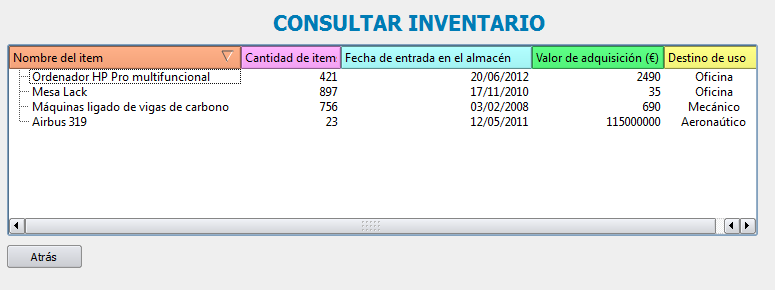
\includegraphics[scale=.6]{imagenes/consultarInventarioImagen.png}
	\caption{Pantalla aproximada de la consulta de inventario}
\end{figure}

								

	% Caso de uso:Consultar nómina.
% Obs: para escribir comas en el texto del primer parámetro se han de encerrar entre {}.
% Revisado por Cristina el día 11/03/2013
\casodeuso{
	% Nombre del caso de uso
	nombre=Consultar nómina.,
	% Objetivo
	objetivo=Consultar la nómina de un empleado.,
	% Entradas
	entradas=Mes del que se desea obtener la nómina.,
	% Precondiciones
	precondiciones=El operador de la aplicación tiene credenciales que le habilitan para realizar dicha operación y tiene una ficha seleccionada.,
	% Salidas
	salidas=El desglose detallado de la nómina.,
	% Postcondiciones en caso de éxito
	postexito=No se realiza ningún cambio en el sistema.,
	% Postcondiciones en caso de error
	posterror=No se realiza ningún cambio en el sistema.,
	% Actores
	actores=Empleados y base de datos.,
}{
	% Tabla de secuencia normal del caso de uso
	\begin{tablasecuencias}
		1 & El usuario selecciona el mes del que se desea consultar la nómina. Si error S-1.
	\end{tablasecuencias}
}{
	% Tabla de secuencia con errores del caso de uso
	\begin{tablasecuencias}
		S-1 & No se han encontrado los datos de la nómina seleccionada. Se muestra un mensaje de error por pantalla dando la opción de reintentar o volver al menú principal de la aplicación.
	\end{tablasecuencias}
}

	\srsfuncion{Configurar nómina}
	Función que debe permitir confeccionar y almacenar las nóminas mensuales de cada empleado de la compañía según las incidencias que se hayan producido en el último mes.
						
	\begin{enumerate}
		\item \textit{Prioridad}: alta.
		\item \textit{Entradas}
			\begin{enumerate}
				\item El usuario debe introducir en el campo de incidencias los motivos por los cuales este mes se produce una modificación en la nómina como, por ejemplo, aumentos o disminuciones del salario a causa de horas extras, comisiones, sustituciones, huelgas\ldots
				\item El sueldo del mes deberá ser mayor o igual al salario mínimo establecido por ley.
			\end{enumerate}
		\item \textit{Flujo de operaciones}
			\begin{enumerate}
				\item Una vez que el usuario ha pulsado la pestaña de \verb|Configurar nómina|, tiene que seleccionar el empleado cuya nómina ha de ser modificada. 
				\item A continuación, el usuario rellena de forma obliglatoria el campo de incidencias y confirmará que quiere aplicar los cambios en la nómina del cliente seleccionado.
				\item Por último, se registra la nómina en la base de datos.
			\end{enumerate}
		\item \textit{Respuesta a situaciones no previstas}
			\begin{enumerate}
				\item Si no se puede establecer conexión con la base de datos: se muestra un mensaje de error y se da la opción de reintentar o abortar el proceso.
				\item Si no se puede registrar la nómina: anular la operación y volver a la página principal del sistema.
			\end{enumerate}					
	\end{enumerate}
								

	\srsfuncion{Consultar ficha de clientes}
	Esta función permite consultar la relación de clientes de la compañía, así como obtener detalles sobre los servicios contratados y los datos personales del usuario. Esto le otorga a los diseñadores --y finalmente a los usuarios-- de esta función una fuerte responsabilidad en el tratamiento de la información.

	\begin{enumerate}
		\item \textit{Prioridad}: alta.
		\item \textit{Entradas}\\
			Al menos uno de los siguientes: identificador personal del cliente (ver \nameref{srs:idpersonal}); nombre o apellidos; o número de vuelo.
			\begin{enumerate}
				\item El identificador personal será validado de acuerdo a las especificaciones de su formato. El tipo de identificador ha de ser seleccionado previamente.
				\item El nombre y los apellidos han de cumplir las condiciones especificadas en este documento, así como el número de vuelo.
			\end{enumerate}
		\item \textit{Flujo de operaciones}
			\begin{enumerate}
				\item Se muestra un formulario de búsqueda, permitiendo al usuario rellenar los campos y ejecutar la petición.
				\item Si no hay resultados se muestra un mensaje; en caso contrario se muestra una pantalla con lista de clientes incluyendo identificador, nombre y apellidos y fecha del último vuelo (si hubiese).
				\item Cuando el usuario seleccione un cliente se mostrará una pantalla con la información detallada del mismo.
			\end{enumerate}
		\item \textit{Respuesta a situaciones no previstas}
			\begin{enumerate}
				\item Si no se puede realizar la búsqueda en la base de datos: informar del error y restablecer el sistema para que se pueda reintentar la operación.
				\item Si no se puede obtener la información de la base de datos: informar al cliente y quedarse en la última pantalla funcional.
			\end{enumerate}
		\item \textit{Relación con otras funciones}\\
		La función está relacionada con \nameref{fun:editarcliente} y \nameref{fun:registrarse} (en la gestión interna) y \nameref{fun:bajacliente}. Se puede utilizar los formularios de consulta para la edición en el \verb|Editar cliente| interno.
	\end{enumerate}

	% Caso de uso: modificar items inventario.
% Obs: para escribir comas en el texto del primer parámetro se han de encerrar entre {}.

% Revisado por Juanan el día 11/03/2013

\casodeuso{
	% Nombre del caso de uso
	nombre=Modificar inventario,
	% Objetivo
	objetivo={Permite modificar diversos datos(Cantidad, precio, imagen, \ldots) , sobre el material registrado en el inventario de la empresa.},
	% Entradas
	entradas=La nueva información sobre el material.,
	% Precondiciones
	precondiciones={El operador de la aplicación tiene credenciales que le habilitan para realizar dicha operación. El servidor que hospeda la base de datos de inventario está operativo.},
	% Salidas
	salidas=El inventario de la empresa modificado en función de los cambios registrados.
	% Postcondiciones en caso de éxito
	postexito=El material registrado en el inventario se actualiza de acuerdo a los datos introducidos.,
	% Postcondiciones en caso de error
	posterror=No se realiza ningún cambio en el sistema.,
	% Actores
	actores=Personal de administación y mecánico.,
}{
	% Tabla de secuencia normal del caso de uso
	\begin{tablasecuencias}
		1 & Se extrae de la base de datos el inventario con los elementos disponibles. Si error S-1. \\
		2 & Se muestra una lista ordenada según el criterio configurado y permite la búsqueda y filtrado.\\
		3 & El usuario añade, elimina elementos del inventario o modifica sus propiedades. Si error S-2.\\
		4 & El usuario confirma que desea hacer permanentes los cambios realizados. Si error S-3.
	\end{tablasecuencias}
}{
	% Tabla de secuencia con errores del caso de uso
	\begin{tablasecuencias}
		S-1 & Si no se puede conectar con la base de datos, se muestra un mensaje de error y vuelve al menú principal.\\
		S-2 & Si algun campo modificado contiene un dato o formato erroneo se avisa y se vuelve a 2 de la secuencia normal de uso. \\
		S-3 & Si no se puede conectar con la base de datos, se muestra un mensaje de error. Se ofrece la posibilidad de reintentar o volver al listado de inventario.
	\end{tablasecuencias}
}


	\srsfuncion{Realizar mantenimiento}
	Esta función debe permitir registrar la información sobre un mantenimiento realizado.

\begin{enumerate}
	\item \textit{Prioridad}: alta.
	\item \textit{Entradas}
	\begin{enumerate}
		\item La información introducida deberá componerse únicamente de carácteres alfabéticos latinos, acentuados o no, dígitos, espacios y otros signos de puntuación.
		\item La cantidad de items del inventario utilizados deberá ser, para cada tipo de item, menor o igual que el número de items disponibles.
	\end{enumerate}
	\item \textit{Flujo de operaciones}
	\begin{enumerate}
		\item Se muestra por pantalla un listado de los mantenimientos programados para el usuario, ordenados por fecha por defecto.
		\item El usuario selecciona un mantenimiento e introduce el informe completo de la operación y de los resultados de ésta. Además, deberá seleccionar una opción \verb|Mantenimiento completado| en caso de que el mantenimiento haya podido finalizarse con éxito. Una vez que haya introducido toda la información detallada del mantenimiento, deberá pulsar en el botón \verb|Guardar|.
		\item A continuación, se muestra por pantalla el listado del material mecánico disponible en el inventario de la empresa. El usuario seleccionará los items que haya utilizado en el mantenimiento e indicará, para cada uno de ellos, la cantidad utilizada. Cuando haya terminado, deberá pulsar en el botón \verb|Guardar|.
		\item Se muestra un mensaje confirmando el registro del mantenimiento.
	\end{enumerate}
	\item \textit{Respuesta a situaciones no previstas}
	\begin{enumerate}
		\item Si no se puede acceder a la base de datos: se muestra un mensaje de error por pantalla y regresa a la página anterior.
	\end{enumerate}

\end{enumerate}

	% Caso de uso: Programar revisión.
% Obs: para escribir comas en el texto del primer parámetro se han de encerrar entre {}.

\casodeuso{
	% Nombre del caso de uso
	nombre=Programar revisión,
	% Objetivo
	objetivo=Permite al personal de mantenimiento programar una revisión para un vehiculo determinado.,
	% Entradas
	entradas={Equipo, herramientas , material y personal necesario. Además de la hora, fecha y vehiculo.},
	% Precondiciones
	precondiciones={Disponibilidad de del vehiculo, así como del peresonal necesario.},
	% Salidas
	salidas=Confirmación adjuntando todos los detalles de la revisión,
	% Postcondiciones en caso de éxito
	postexito={Quedarán asignado un hangar para llevar a cabo la revisión, así como registrados los datos correspondientes y reservados para el propósito los recursos humanos y materiales indicados.},
	% Postcondiciones en caso de error
	posterror=No se altera la base de datos.,
	% Actores
	actores=Personal de mantenimiento autorizado.
}{
	% Tabla de secuencia normal del caso de uso
	\begin{tablasecuencias}
		1 & Se escoge fecha y hora.\\
		2 & Se selecciona vehiculo.\\
		3 & Se especifica el material y las herramientas necesarias. Si error S-1.\\
		4 & Se elige al personal de entre los disponibles.\\
		5 & Se da la opción de confirmar operación.
	\end{tablasecuencias}
}{
	% Tabla de secuencia con errores del caso de uso
	\begin{tablasecuencias}
		S-1 & Si alguno de los elementos no se encuentra disponible en el almacén se notificará y vuelve al paso 3 de la secuencia normal.\\
		S-2 & Si no se puede conectar con la base de datos, se muestra un mensaje de error.
	\end{tablasecuencias}
}

	% Caso de uso: registrar entrada de material
% Obs: para escribir comas en el texto del primer parámetro se han de encerrar entre {}.

% Revisado por Cristina el día 11/03/2013

\casodeuso{
	% Nombre del caso de uso
	nombre=Registrar entrada de material,
	% Objetivo
	objetivo=Registrar una entrada de material en el inventario de la empresa.,
	% Entradas
	entradas={Nombre del producto o identificador si es un material previamente registrado, descripción, sección que lo recibe (si procede) y ubicación final.},
	% Precondiciones
	precondiciones=El operador de la aplicación tiene credenciales que le habilitan para realizar dicha operación.,
	% Salidas
	salidas=Adhesivo de inventario con la clave de identificación del material en el sistema (si procede).,
	% Postcondiciones en caso de éxito
	postexito=Se actualiza el inventario de la empresa de acuerdo al registro realizado.,
	% Postcondiciones en caso de error
	posterror=No se realiza ningún cambio en el sistema.,
	% Actores
	actores=El personal de la compañía y la base de datos.,
}{
	% Tabla de secuencia normal del caso de uso
	\begin{tablasecuencias}
		1 & El empleado introduce los datos necesarios del registro. Si error S-1.\\
		2 & Se registran los cambios en el sistema correspondiente. Si error S-2.\\
		3 & Se obtiene una adhesivo impreso para identificar el objeto catalogado (si procede).
	\end{tablasecuencias}
}{
	% Tabla de secuencia con errores del caso de uso
	\begin{tablasecuencias}
		S-1 & El sistema vuelve a 1 de la secuencia normal de uso e indica los campos erróneos.\\
		S-2 & No se puede conectar con la base de datos, se muestra un mensaje de error por pantalla dando la opción de reintentar o volver al menú principal de la aplicación.
	\end{tablasecuencias}
}

	% Caso de uso: Dar de baja cliente.
% Obs: para escribir comas en el texto del primer parámetro se han de encerrar entre {}.

\casodeuso{
	% Nombre del caso de uso
	nombre= Dar de baja cliente,
	% Objetivo
	objetivo={Permitir a un cliente que pueda darse de baja en nuestro sistema borrando todos sus datos de él. Esta acción es obligatoria en cualquier sistema donde se pueda registrar un cliente por la LOPD \textit{(Ley Orgánica de Protección de Datos)}.},
	% Entradas
	entradas={Un personal administrativo acceda a la opción del sistema para dar de baja a un cliente.},
	% Precondiciones
	precondiciones={Que el cliente se haya puesto en contacto con la empresa indicándole que quiere darse de baja en el sistema y haberse registrado como un usuario válido de la aplicación perteneciente al Personal de atención al cliente. Elegir la opción \textit{Dar de baja cliente}.},
	% Salidas
	salidas= {Eliminar al cliente de la base de datos de la empresa.},
	% Postcondiciones en caso de éxito
	postexito={Los datos del cliente habrán desaparecido de la base de datos del sistema, borrándose todo por completo.},
	% Postcondiciones en caso de error
	posterror={Los datos del cliente no se habrán eliminado y seguirán estando en nuestro sistema.},
	% Actores
	actores={El Personal de atención al cliente, el cliente a dar de baja y la base de datos.},
}{
	% Tabla de secuencia normal del caso de uso
	\begin{tablasecuencias}
		1 & El cliente notifica a la empresa que desea darse de baja en su sistema.\\
		2 & El personal administrativo accede al sistema y da a la opción de dar de baja al cliente.\\
		3 & El sistema accede a la base de datos para encontrar al cliente. Si error S-1\\
		4 & Se borran del sistema los datos del cliente. Si error S-2.\\
		5 & Se notifica al cliente de que ha sido dado de baja con éxito.
	\end{tablasecuencias}
}{
	% Tabla de secuencia con errores del caso de uso
	\begin{tablasecuencias}
		S-1 & No se ha encontrado al cliente en la base de datos, por lo que se muestra un mensaje de que el cliente no existe.\\
		S-2 & Si no se ha podido eliminar los datos del cliente se le notifica indicándole que si quiere darse de baja vuelva a realizar la operación.
	\end{tablasecuencias}
}



	% Caso de uso: Programar oferta.
% Obs: para escribir comas en el texto del primer parámetro se han de encerrar entre {}.

\casodeuso{
	% Nombre del caso de uso
	nombre=Programar oferta,
	% Objetivo
	objetivo=Poder crear una nueva oferta para poder mostrarla y darle acceso posteriomente a los clientes.,
	% Entradas
	entradas=Los datos concretos de la oferta.,
	% Precondiciones
	precondiciones=Haber accedido al sistema.,
	% Salidas
	salidas=Crear una oferta que la empresa desea mostrar.,
	% Postcondiciones en caso de éxito
	postexito=Se crea una nueva oferta para promocionar un item y motivar su venta.,
	% Postcondiciones en caso de error
	posterror=No se modifica la lista de ofertas de la empresa.,
	% Actores
	actores=La base de datos y el personal administrativo cuyo rol sea programar., 
}{
	% Tabla de secuencia normal del caso de uso
	\begin{tablasecuencias}
		1 & Rellenar el formulario de una oferta con todos los datos requeridos.\\
		2 & Añadir la oferta a la lista de ofertas de la base de datos de la empresa. Si error S-1.
	\end{tablasecuencias}
}{
	% Tabla de secuencia con errores del caso de uso
	\begin{tablasecuencias}
		S-1 & No se ha podido añadir la oferta a la base de datos, mostrar un mensaje de error y permitir que el usuario pueda volver a intentar añadir la oferta.
	\end{tablasecuencias}
}

	% Caso de uso: Efectuar embarque
% Obs: para escribir comas en el texto del primer parámetro se han de encerrar entre {}.

% Comentario de Aitor, si un cliente no se presenta a un embarque se cancelan todos los billetes asociados a ese cliente.
% Revisado por Juanan el día 12/03/2013

\casodeuso{
	% Nombre del caso de uso
	nombre=Efectuar embarque,
	% Objetivo
	objetivo=Registrar el embarque del pasajero.,
	% Entradas
	entradas=El número de vuelo y el número de reserva del pasajero.,
	% Precondiciones
	precondiciones=El operador de la aplicación tiene credenciales que le habilitan para realizar dicha operación y un billete válido,
	% Salidas
	salidas=Confirmación de que el pasajero pasa el control de seguridad con éxito y ha embarca en el avión.,
	% Postcondiciones en caso de éxito
	postexito=Se registra el embarque del pasajero.,
	% Postcondiciones en caso de error
	posterror=No se realiza ningún cambio en el sistema.,
	% Actores
	actores=El personal de la compañía presente en el aeropuerto y la base de datos.
}{
	% Tabla de secuencia normal del caso de uso
	\begin{tablasecuencias}
		1 & El usuario introduce el número de vuelo y el número de reservar del pasajero. Si error S-1.\\
		2 & Se comprueba la reserva y se actualiza la base de datos. Si error S-2.		
	\end{tablasecuencias}
}{
	% Tabla de secuencia con errores del caso de uso
	\begin{tablasecuencias}
		S-1 & Alguno de los campos introducidos por el usuario no es válido. Se muestra un mensaje de error y se vuelve a 1 de la secuencia normal de uso indicando los datos erroneos. \\
		S-2 & No se ha podido conectar con la base de datos. Se muestra un mensaje de error y se ofrece la posibilidad de reintentar.
	\end{tablasecuencias}
}


	% Caso de uso: ver incidencias del sistema.
% Obs: para escribir comas en el texto del primer parámetro se han de encerrar entre {}.

\casodeuso{
	% Nombre del caso de uso
	nombre=Ver incidencias del sistema,
	% Objetivo
	objetivo={Permite a los supervisores informáticos del sistema inspeccionar el correcto funcionamiento del \software y responder a comportamientos erróneos del mismo que hayan sido detectados, a partir de los registros que este genera.},
	% Entradas
	entradas={El nombre de registro que se quiere consultar.},
	% Precondiciones
	precondiciones={El operador de la aplicación está debidamente registrado y posee credenciales que le habilitan para realizar esta operación.},
	% Salidas
	salidas={Archivos de registro del sistema solicitados.},
	% Postcondiciones en caso de éxito
	postexito={},
	% Postcondiciones en caso de error
	posterror={El sistema central no habrá sufrido cambios.},
	% Actores
	actores={Personal de \textit{Servicios Informáticos} y supervisores del sistema con autorización para ello.},
}{
	% Tabla de secuencia normal del caso de uso
	\begin{tablasecuencias}
		1 & Los archivos de registro del servidor central y los errores reportados por las aplicaciones cliente componen una serie de archivos de texto en el servidor central. Esos archivos podrán ser consultados dando acceso a su ubicación en el sistema de archivos del servidor central.
		% De momento, ¿para qué complicarlo?
	\end{tablasecuencias}
}{
	% Tabla de secuencia con errores del caso de uso
	\begin{tablasecuencias}
		S-1 & Las secuencias alternativas son las que determine el método de acceso al servidor.
	\end{tablasecuencias}
}


	% Gestión externa
	\subsection{Gestión externa} \vspace{.5cm}

	\begin{sidewaysfigure}
		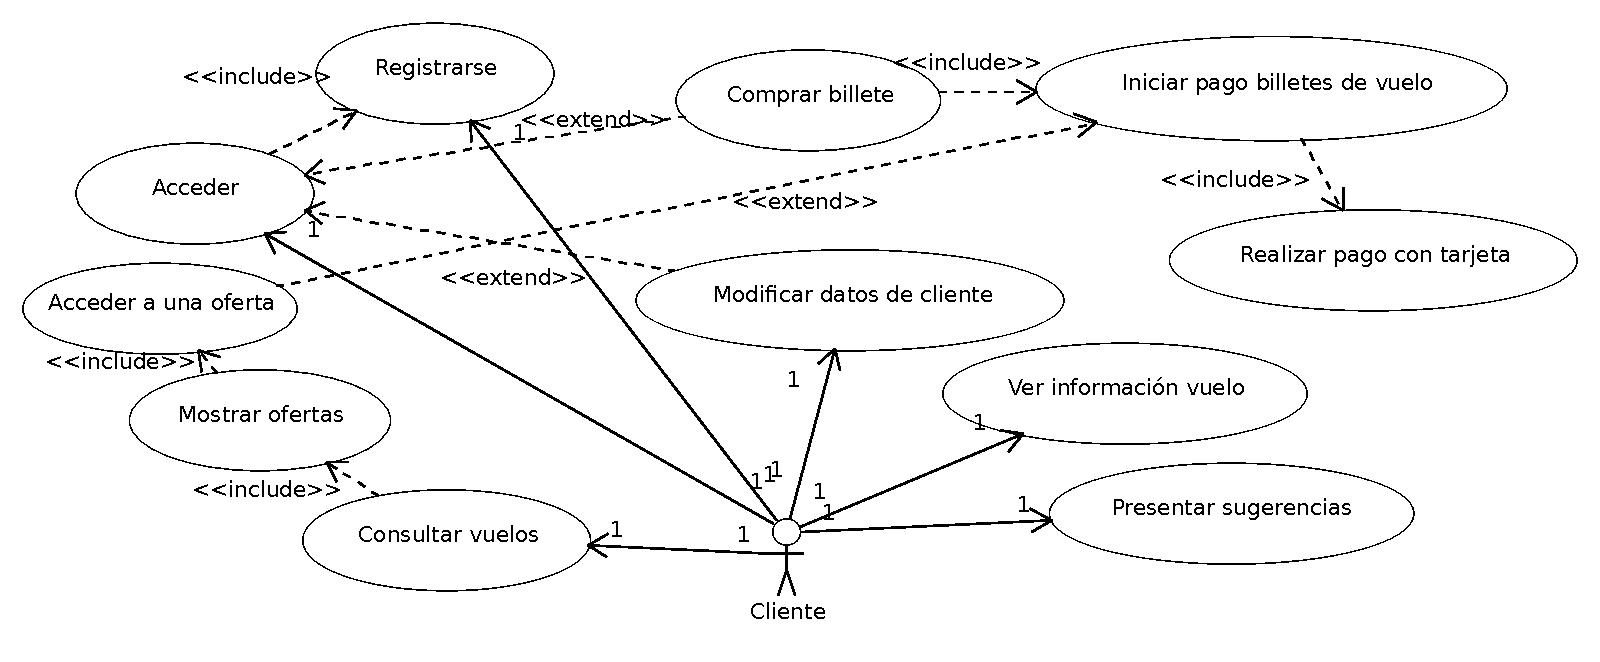
\includegraphics[scale=.93]{diagramas/gestionexterna.pdf}
		\caption{Diagrama de gestión externa}
	\end{sidewaysfigure}

	% Revisado por Cristina el día 12/03/2013

\srsfuncion{Acceder web} \label{fun:accederge}
	Función que permite hacer \textit{\gls{Login}} al usuario (en este caso cliente de la compañía aérea) para poder acceder al sistema.
		
	\begin{enumerate}
		\item \textit{Prioridad}: media.
		\item \textit{Entradas}
		\begin{enumerate}
			\item El nombre de usuario y la contraseña son campos obligatorios a introducir.
			\item En el campo contraseña son válidos los caracteres ASCII imprimibles.
		\end{enumerate}
		\item \textit{Flujo de operaciones}
		\begin{enumerate}
			\item Se muestran por pantalla dos campos a rellenar: uno para introducir el id del usuario y otro para escribir la contraseña.
			\item El usuario selecciona la opción de acceder al sistema.
		\end{enumerate}
		\item \textit{Respuesta a situaciones no previstas}
		\begin{enumerate}
			\item Si algún campo introducido no es válido, se indica y se da la opción de introducirlo de nuevo. Existe un límite de 5 intentos de acceso fallido en un periodo de tiempo corto (15 minutos).
		\end{enumerate}
	
\end{enumerate}

	
% Revisado por Juanan el día 12/03/2013

\srsfuncion{Registrarse} \label{fun:registrarse}
	Esta función crea una nueva cuenta de cliente asociada a un visitante de la página web de la compañía.

	\begin{enumerate}
		\item \textit{Prioridad}: alta.
		\item \textit{Entradas}\\
			Será necesario introducir los siguiente datos: nombre y apellidos, código de identificación personal y una cuenta de correo electrónico. En cambio, la introducción de los siguientes datos es opcional: teléfono, dirección.

			\begin{enumerate}
				\item El código de idenficación personal será validado de acuerdo a las especificaciones de su formato.
				\item El nombre y los apellidos deberán contener únicamente carácteres alfabéticos latinos, acentuados o no, y espacios.
				\item La dirección de correo ha de seguir el formato \verb|nombre@dominio.com|. Se comprobará, en la medida de los posible, la autenticidad del servicio de correo introducido.
				\item El número de teléfono debe ser una secuencia de 9 dígitos. % Telefono español?
				\item La dirección debe cumplir los requisitos establecidos en \nameref{srs:direccionpostal}.
			\end{enumerate}
		
		\item \textit{Flujo de operaciones}
			\begin{enumerate}
				\item Se muestra un formulario con los distintos campos anteriormente detallados para que el usuario los rellene. 
				\item Se solicita además el paso de un \gls{captcha} por motivos de seguridad. Hasta que éste no sea superado no se permitirá continuar con el registro.
				\item Se muestran los derechos del usuario y las condiciones del servicio que deberán ser aceptadas, no pudiendo seguir con el registro hasta entonces.
				\item Cuando ha realizado correctamente todos los pasos anteriores debe \verb|Confirmar registro| y se procede al registro en la base de datos central.
			\end{enumerate}
		\item \textit{Respuesta a situaciones no previstas}
			\begin{enumerate}
				\item Si alguno de los datos no es válido o se ha dejado sin rellenar algún campo obligatorio se mostrará como erróneo y se dará la opción al usuario de modificarlo.
				\item Si no se puede registrar al usuario en la base de datos: informar al usuario e indicarle que puede volverlo a intentar en otro momento.
			\end{enumerate}
		\item \textit{Relación con otras funciones}\\
			Este caso es útil para todos aquellos que requieran un usuario registrado, como \verb|Acceder web| o aunque no lo requieran como \nameref{fun:iniciarpago}.
	\end{enumerate}

	\srsfuncion{Editar cliente} \label{fun:editarcliente}
	Esta función debe mostrar al usuario su perfil y permitirle la modificación del mismo.

\begin{enumerate}
	\item \textit{Entradas}
	\begin{enumerate}
		\item Las opciones que admiten modificación son: Contraseña, domicilio, dirección de correo electrónico, tarjeta de crédito asociada.
		\item La contraseña estará formada por entre 8 y 16 caracteres alfanúmericos.
		\item El código postal del domicilio ha de estar formado por 5 cifras.
		\item Se comprobará la correción del correo electrónico mediante un e-mail de verificación.
		\item Se verificará algoritmicamente los 20 digitos de numeración de la tarjeta de crédito, así como la validez de la misma junto con la fecha de caducidad y el código \gls{CVV2}.
	\end{enumerate}
	\item \textit{Flujo de operaciones}
	\begin{enumerate}
		\item Se muestra un formulario con los campos modificables actuales del usuario.
		\item El usuario modifica al menos uno de los diferentes campos. La válided de los campos modificados se comprueba al pulsar el botón Guardar Cambios.
		\item Si se encuentra algún dato erroneo se informa de ello. Si se verificán los datos modificados se confirma la operación, actualizando la \gls{base_de_datos}.
		\item Se muestra el perfil de usuario resultado de la modificación.
	\end{enumerate}
	\item \textit{Respuesta a situaciones no previstas}
	\begin{enumerate}
		\item Si no se puede acceder o modificar a la base de datos: informa de la no disponibilidad temporal al usuario.
	\end{enumerate}
\end{enumerate}

	% Caso de uso: consultar vuelos.
% Obs: para escribir comas en el texto del primer parámetro se han de encerrar entre {}.

\casodeuso{
	% Nombre del caso de uso
	nombre=Consultar vuelos,
	% Objetivo
	objetivo={Mostrar al cliente la relación de vuelos operados por la compañía, pudiendo filtrar resultados y buscar por diferentes criterios; permitiendo además obtener información detallada de los vuelos seleccionados.},
	% Entradas
	entradas={Opcionalmente las que correspondan a los filtros (aeropuertos de origen y destino, número de escalas, fecha y hora, precio del billete\ldots). En última instancia, vuelo seleccionado.},
	% Precondiciones
	precondiciones={La información de vuelos ha sido previamente introducida en el sistema, así como los criterios configurados.},
	% Salidas
	salidas={Una lista filtrada de vuelos y, al seleccionar uno de ellos, información detallada del mismo.},
	% Postcondiciones en caso de éxito
	postexito=El cliente puede acceder a la compra de billetes del vuelo seleccionado.,
	% Postcondiciones en caso de error
	posterror={Una pantalla de notificación de error, en la medida de lo posible.},
	% Actores
	actores={Clientes de la compañía, base de datos.},
}{
	% Tabla de secuencia normal del caso de uso
	\begin{tablasecuencias}
		1 & Se muestra una lista de vuelos ordenados por un criterio asignado por defecto. Si error S-1. \\
		2 & El usuario puede filtrar los resultados según diferentes reglas, aparecerá una lista reducida de vuelos (incluso nula).\\
		3 & Seleccionando uno de ellos se accederá a la información especializada en ese servicio, dando acceso a la adquisición de billetes. 
	\end{tablasecuencias}
}{
	% Tabla de secuencia con errores del caso de uso
	\begin{tablasecuencias}
		S-1 & Si no se puede acceder al servidor central o no se puede obtener la información de vuelos, informar al usuario.
	\end{tablasecuencias}
}

	% Caso de uso: Mostrar ofertas.
% Obs: para escribir comas en el texto del primer parámetro se han de encerrar entre {}.

\casodeuso{
	% Nombre del caso de uso
	nombre=Mostrar ofertas.,
	% Objetivo
	objetivo=Mostrar las ofertas actuales a los clientes con el fin de incentivar su compra.,
	% Entradas
	entradas=El cliente podrá elegir una oferta entre las que se muestran.,
	% Precondiciones
	precondiciones=Haber accedido a la página web de la compañía.,
	% Salidas
	salidas=Las ofertas actuales.,
	% Postcondiciones en caso de éxito
	postexito=Muestra las ofertas actuales de la compañía.,
	% Postcondiciones en caso de error
	posterror=No se modifica la página web.,
	% Actores
	actores=Cualquier usuario que acceda a la página web y la base de datos.
}{
	% Tabla de secuencia normal del caso de uso
	\begin{tablasecuencias}
		1 & Acceder a la base de datos. Si error S-1.\\
		2 & Muestra por pantalla las ofertas de la compañía.\\
		3 & Si el cliente accede a una oferta en concreto, se rediccionará a esa oferta a través de \textit{Acceder a la oferta}. Si error S-2.
	\end{tablasecuencias}
}{
	% Tabla de secuencia con errores del caso de uso
	\begin{tablasecuencias}
		S-1 & No se puede acceder a la base de datos. No se cargan las ofertas y se muestra la pantalla de la página web sin las ofertas.\\
		S-2 & Si no se ha podido rediccionar a la oferta elegida se mostrará un mensaje por pantalla indicando que la oferta no es accesible en estos momentos.
	\end{tablasecuencias}
}

	\srsfuncion{Acceder a una oferta}
	Esta función debe mostrar una oferta específica elegida por el cliente y podrá dar la opción de comprar lo ofertado.
	
\begin{enumerate}
	\item \textit{Prioridad}: media.
	\item \textit{Entradas}
	\begin{enumerate}
		\item Los datos detallados de la oferta tendrán que estar en el mismo idioma en el que estaba el resumen de la oferta.
	\end{enumerate}
	\item \textit{Flujo de operaciones}
	\begin{enumerate}
		\item La oferta aparecerá descrita detalladamente especificando el/los artículo/s ofertados, por lo que si el usuario estuviese interesado en ella podrá comprar y pagar la oferta.
		\item Si la oferta consta de varias opciones de compra, el cliente podrá elegir entre todas las que haya.
		\item Si el cliente pulsa el botón \verb|Comprar|, se le redireccionará al proceso de realizar pago para que lo efectúe.
	\end{enumerate}
	\item \textit{Respuesta a situaciones no previstas}
	\begin{enumerate}
		\item Si al intentar acceder a una oferta el sistema falla, se mostrará un mensaje de error por pantalla informando de que los datos de esta oferta pueden ser que estén dañados o que simplemente no esté ya disponible. 
	\end{enumerate}
\end{enumerate}

	% Caso de uso: Presentar reclamacion
% Obs: para escribir comas en el texto del primer parámetro se han de encerrar entre {}.

\casodeuso{
	% Nombre del caso de uso
	nombre=Presentar reclamaciones,
	% Objetivo
	objetivo= Presentar una reclamación por parte del cliente.,
	% Entradas
	entradas= Motivo de la queja y detallado de la misma.,
	% Precondiciones
	precondiciones=Intención por parte del usuario de transmitir una sugerencia o queja a la empresa.,
	% Salidas
	salidas=Confirmación del envio y número asociado a la reclamación.,
	% Postcondiciones en caso de éxito
	postexito=La notificación es enviada correctamente al departamento correspondiente.,
	% Postcondiciones en caso de error
	posterror=No se tramita la petición.,
	% Actores
	actores=Cliente-usuario de interfaz web.,
}{
	% Tabla de secuencia normal del caso de uso
	\begin{tablasecuencias}
		1 & Completar todos sus datos, el motivo de la reclamación, y detalles de la misma. Si error S-1. \\
		2 & Muestra número asignado a la reclamación junto a la confirmación de que la reclamación ha sido tramitada y en breve será atendia por el departamento correspondiente. Si error S-2. 
		
	\end{tablasecuencias}
}{
	% Tabla de secuencia con errores del caso de uso
	\begin{tablasecuencias}
		S-1 & Los campos de datos están incompletos. Indicar los campos erróneos o vacíos.\\
		S-2 & Si no se han podido transmitir los datos de la reclamación a nuestra base de datos se indicará un mensaje de que la operación ha sido fallida debido a errores técnicos y de que se vuelva a intentar.
	\end{tablasecuencias}
}


	\srsfuncion{Comprar billete}
	Esta función debe permitir al usuario iniciar el proceso de compra de billetes de un vuelo seleccionado.		

	\begin{enumerate}
		\item \textit{Entradas}
			\begin{enumerate}
				\item El nombre y apellidos de los pasajeros deberá contener únicamente carácteres alfabéticos latinos, acentuados o no, y espacios.
				\item La selección de asientos se realizará en función de los asientos disponibles en el momento de la compra de los billetes.
				\item Los datos de la persona que paga serán, de momento, nombre y apellidos,  que deberá contener únicamente carácteres alfabéticos latinos, acentuados o no, y espacios.							
			\end{enumerate}
		\item \textit{Flujo de operaciones}
			\begin{enumerate}
				\item Se muestra por pantalla el itinerario del vuelo a comprar, el precio total a pagar, desglosándolo en la parte correspondiente al pasajero, la tarifa, los impuestos, tasas y suplementos de transporte.
				\item Se muestran los asientos disponibles del avión en el momento de la compra, dando la opción al cliente de reservar los asientos que desee en su vuelo.
				\item El cliente deberá introducir los datos (nombre y apellidos) de la persona que realizará el pago de billetes (no tiene porqué ser un pasajero). Si todo ha ido correctamente se habilita un botón \verb|Continuar| y se redirecciona a~\ref{fun:iniciarpago}.
			\end{enumerate}
		\item \textit{Respuesta a situaciones no previstas}
			\begin{enumerate}
				\item Si no se puede mostrar la información del vuelo seleccionado: se muestra un mensaje de error por pantalla y se vuelve a la página anterior.
				\item Si alguno de los datos no es válido: se muestran los campos erróneos y se da la opción de editarlos de nuevo.
				\item Si algún campo no se ha rellenado: se muestra un mensaje indicando que es obligatorio completarlo.
				\item Si no se puede realizar la reserva de asientos: se muestra el error y sigue la secuencia normal.
				\item Si no se puede conectar con la base de datos y, por tanto, no se puede realizar la compra,  se mostrará un mensaje indicando que el proceso de pago ha sido interrumpido. Se vuelve a la página principal de la aplicación.
			\end{enumerate}
	\end{enumerate}
								

	\srsfuncion{Iniciar pago billetes de vuelo} \label{fun:iniciarpago}
	Esta función debe permitir al usuario adquirir un billete de vuelo, de acuerdo a la selección previa.

\begin{enumerate}
	\item \textit{Entradas}
	\begin{enumerate}
		\item Los detalles completos de la selección del vuelo.
	\end{enumerate}
	\item \textit{Flujo de operaciones}
	\begin{enumerate}
		\item Se muestra por pantalla los datos completos del vuelo, siempre que no se haya excedido el tiempo de reserva desde la selección del billete.
		\item Se muestra las claúsulas de las leyes de protección de datos para que el usuario las acepte. Hasta que no lo haga no continúa el proceso de pago.
		\item Se redirecciona a \nameref{fun:pagotarjeta}.
	\end{enumerate}
	\item \textit{Respuesta a situaciones no previstas}
	\begin{enumerate}
		\item Si no se puede acceder a la base de datos para almacenar la información: se muestra un mensaje de error por pantalla informando de que el proceso de pago se ha interrumpido. Se vuelve a la página anterior.
	\end{enumerate}
\end{enumerate}

	% Revisado por Juanan el día 12/03/2013

\srsfuncion{Realizar pago con tarjeta} \label{fun:pagotarjeta}
	Esta función permite al usuario finalizar el proceso de compra del billete realizando el pago con tarjeta de crédito o débito.

\begin{enumerate}
	\item \textit{Prioridad}: alta.
	\item \textit{Entradas}
	\begin{enumerate}
		\item El nombre del usuario (nombre y apellidos) deberán contener únicamente carácteres\break alfabéticos latinos, acentuados o no, y espacios.
		\item El número de la tarjeta deberá ser una secuencia de 4 bloques de 4 dígitos, todos ellos enteros mayores o iguales que 0.
		\item El código CCV deberá ser una secuencia de 3 dígitos mayores o iguales que 0.
		\item La fecha de caducidad  ser una secuencia de 5 caracteres compuesta por: 2 dígitos para indicar el mes (en el rango 01-12) , una barra `/'  y otros 2 dígitos para indicar el año, que serán las dos últimas cifras del mismo.
	\end{enumerate}
	\item \textit{Flujo de operaciones}
	\begin{enumerate}
		\item Se muestra por pantalla una tabla con los datos de la tarjeta a completar (nombre y apellidos, número, código CCV y fecha de caducidad). Una vez completos, se habilita la opción \verb|Confirmar|.
		\item Se transfieren los datos de la tarjeta a la empresa emisora de las mismas para que compruebe si los datos son correctos y la tarjeta está operativa. En este caso, se enviará al instante un mensaje a la compañía indicando que los datos introducidos por el usuario son válidos.
		\item Si está todo correcto, se da la opción de imprimir en el momento la tarjeta de embarque o guardarla como pdf para imprimirla en otro momento.
	\end{enumerate}
	\item \textit{Respuesta a situaciones no previstas}
	\begin{enumerate}
		\item Si no se puede acceder a la base de datos para almacenar la información: se muestra un mensaje de error por pantalla informando de que el proceso de pago se ha interrumpido. Se vuelve a la página anterior.
		\item Si alguno de los datos no es válido: se muestran los campos erróneos y se da la opción de editarlos de nuevo.
		\item Si algún campo no se ha rellenado: se muestra un mensaje indicando que es obligatorio completarlo.
		\item Si la tarjeta está inhabilitada por algún motivo: se muestra un error indicando que el pago no ha podido completarse porque la tarjeta está bloqueada. Se cancela la operación y se vuelve a la página principal de la aplicación.
		\item Si los datos de la tarjeta no son válidos: se muestra un error indicando que el pago no ha podido completarse y se da la opción al usuario de modificar los datos introducidos al principio de la operación.
	\end{enumerate}
	\item \textit{Relación con otras funciones}\\
		Esta función está relacionada con \nameref{fun:consultaroferta}, \nameref{fun:mostrarofertas}, \nameref{fun:iniciarpago} y \nameref{fun:comprarbillete}.	
\end{enumerate}

	% Caso de uso: ver información de vuelo
% Obs: para escribir comas en el texto del primer parámetro se han de encerrar entre {}.

\casodeuso{
	% Nombre del caso de uso
	nombre=Ver información de vuelo contratado,
	% Objetivo
	objetivo=Mostrar al usuario la información de sus vuelos contratados.,
	% Entradas
	entradas=,
	% Precondiciones
	precondiciones=El usuario ha iniciado sesión correctamente en la interfaz web.,
	% Salidas
	salidas=Información detallada de la reserva(número de vuelo, fecha y hora, número de plaza, terminales de salida y de llegada\ldots)},
	% Postcondiciones en caso de éxito
	postexito=No se realiza ningún cambio en el sistema.,
	% Postcondiciones en caso de error
	posterror=No se realiza ningún cambio en el sistema.,
	% Actores
	actores=Cliente-usuario de interfaz web.
}{
	% Tabla de secuencia normal del caso de uso
	\begin{tablasecuencias}
		1 & Muestra listado detallo de los vuelos contratados. Si no disponibles S-1.\\
		2 & Ofrece la opción de seleccionar e imprimir la información de los vuelos mostrados.
	\end{tablasecuencias}
}{
	% Tabla de secuencia con errores del caso de uso
	\begin{tablasecuencias}
		S-1 & Si no se puede conectar con la base de datos se muestra mensaje  de tipo \textit{información no disponible temporalmente} y se vuelve al menú principal de la aplicación.
	\end{tablasecuencias}
}

	
\end{document}
